\documentclass[10pt,a4paper,oneside]{article}
\usepackage[utf8]{inputenc}
\usepackage[english]{babel}
\usepackage{amsmath}
\usepackage{amsfonts}
\usepackage{amssymb}
\usepackage{graphicx}
%personal preferences for hyperlinks 
\usepackage[hidelinks]{hyperref}
\hypersetup{colorlinks=true}
%changing the separator before a figure's caption
\usepackage[labelsep=space]{caption}
%changing the margins 
\usepackage[left=2.5cm, top=2.5cm,right=2.5cm, bottom=2.5cm]{geometry}

%document title, no date 	
\title{Using the University of Sheffield licensed XE 2017 Intel Compilers with Visual Studio 2015 Community for Windows}
\date{}

\begin{document}
\maketitle
This document explains how to install and use the University of Sheffield site licensed versions of Intel Fortran, C, and C++ compilers with the free Microsoft Visual Studio 2015 Community Edition. 

\section*{Important Licensing Note}
Intel Compilers are licensed using network based licenses at the University of Sheffield. Therefore, you need to be connected to the University network for both installation of the software and during compilation of source code . There is no need to be connected to the University network during program runtime. If working off-site you need to be connected to the University VPN client.

Our licenses support up to 5 concurrent compilations site-wide. Such a number of licenses should be sufficient for research purposes and \textbf{not for teaching large classes}. 

The University of Sheffield has site licenses for a range of compilers, some of which are suitable for teaching purposes. For more information please refer to the Fortran, C, and C++ sections of the \href{http://rse.shef.ac.uk/resources/}{University Research Software Engineering Resources} page. 

\section*{Software requirements}
In order to use the Intel C/C++ and Intel Visual Fortran Compilers as part of the Intel Parallel Studio XE 2017  one of the following applications is required prior installation:
\begin{itemize}
\item Microsoft Visual Studio 2015 Community Edition or higher with C++ component installed (please note that the C++ component is not installed by default but need to done using the Custom option during installation).
\item Microsoft Visual Studio 2013 Community Edition with C++ component
\item Microsoft Visual Studio 2012 Professional Edition with C++ component
\end{itemize}
For  more detailed system and software requirements consult the \href{https://software.intel.com/en-us/articles/intel-parallel-studio-xe-release-notes}{release notes}.
\newpage
\section*{Before installing the compilers}
If you have not got a supported Microsoft Visual Studio version already installed in your computer, download and install \href{https://www.microsoft.com/en-us/download/details.aspx?id=48146}{Microsoft Visual Studio 2015} Community edition. 

During installation \textbf{you must install the C++ components} of the Microsoft Visual Studio 2015 Community edition by selecting the \textbf{Custom} option (Fig. \ref{fig:VS1}).
\begin{figure}[!ht]
\centering
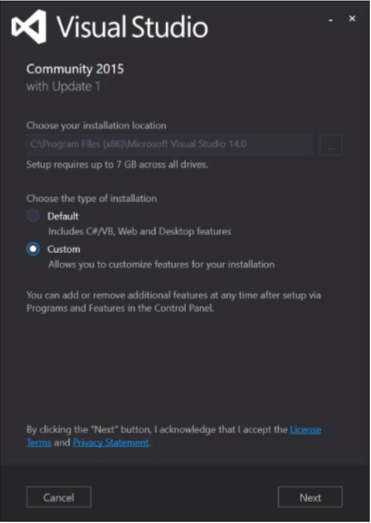
\includegraphics[scale=0.45]{VS1.png}
\caption{}
\label{fig:VS1}
\end{figure}

Expand the \textbf{Programming languages} tree and select \textbf{Visual C++} (Fig. \ref{fig:VS2}).
\begin{figure}[ht]
\centering
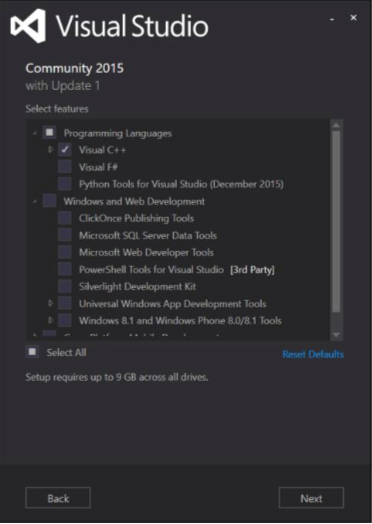
\includegraphics[scale=0.45]{VS2.png}
\caption{}
\label{fig:VS2}
\end{figure}

\section*{Installing the Intel Compiler Suite}
In order to install the Intel Compiler Suite you need to make sure that you are connected to the University Network. Then run the installer which will guide you through the installation process. 

At the Activation screen, select \textbf{Choose alternative activation} (Fig. \ref{fig:VS3}).
\begin{figure}[ht]
\centering
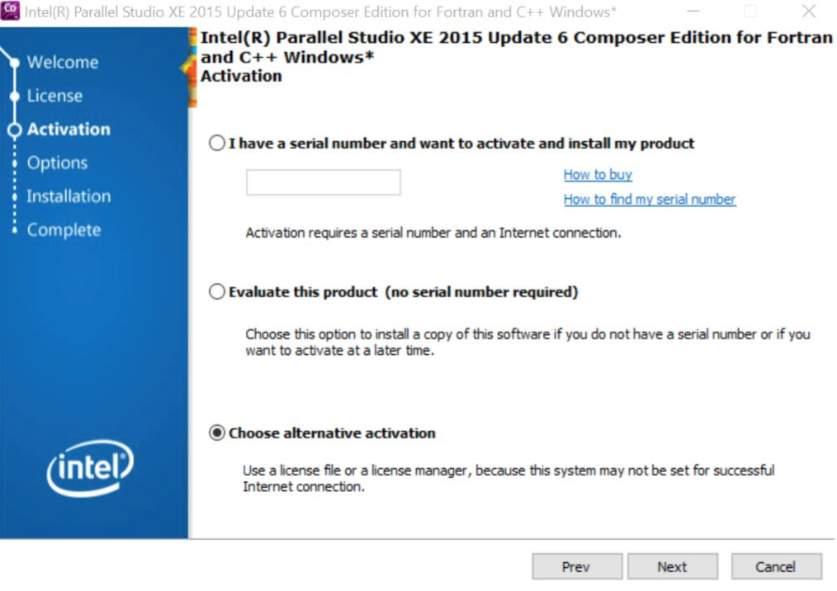
\includegraphics[scale=0.4]{VS3.png}
\caption{}
\label{fig:VS3}
\end{figure}
At the following screen, select \textbf{use a licence manager} (Fig. \ref{fig:VS4}).
\begin{figure}[ht]
\centering
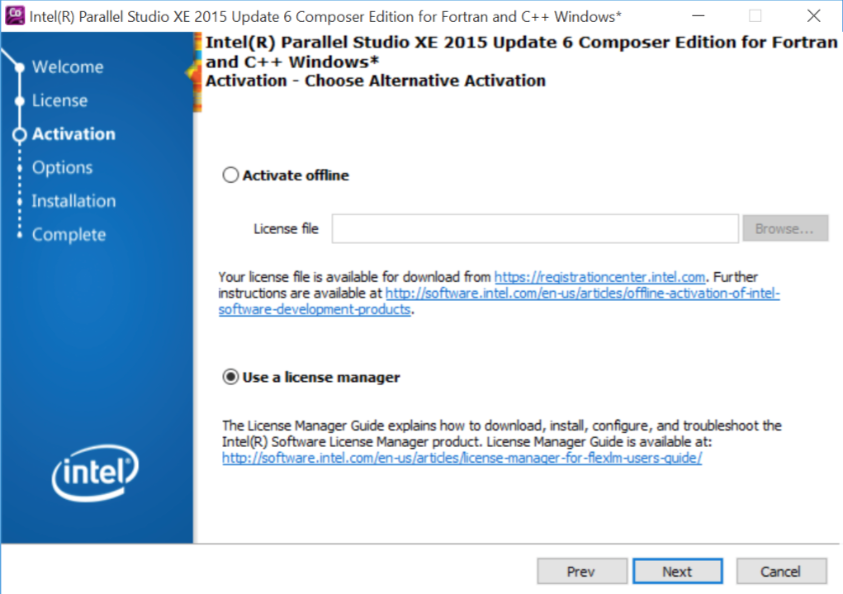
\includegraphics[scale=0.4]{VS4.png}
\caption{}
\label{fig:VS4}
\end{figure}

When prompted, enter the following information (Fig. \ref{fig:VS5})
\begin{itemize}
\item \textbf{Host name:} licserv.shef.ac.uk
\item \textbf{Port:} 28518
\end{itemize}
\begin{figure}[ht]
\centering
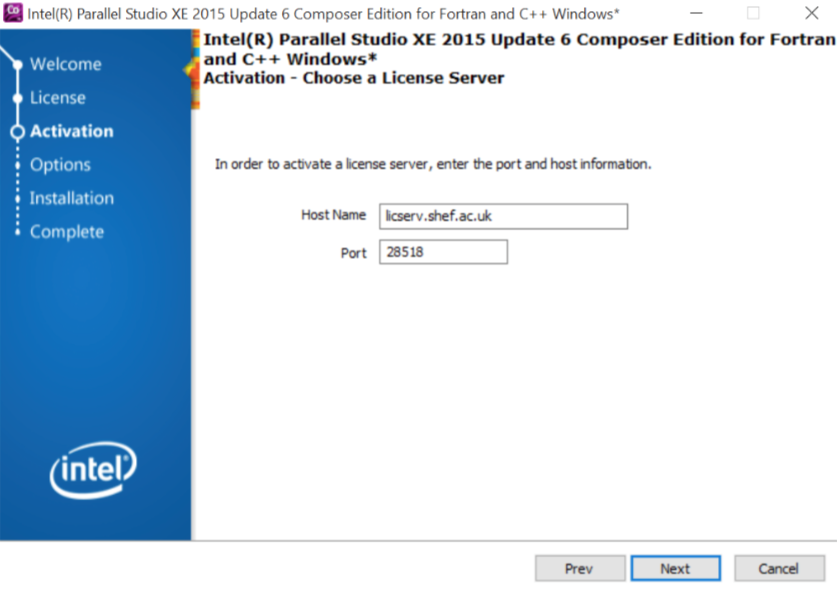
\includegraphics[scale=0.4]{VS5.png}
\caption{}
\label{fig:VS5}
\end{figure}

\subsection*{Creating a console-based Intel Fortran project}
Launch Visual Studio 2015 Community Edition and create a new Project. You should se Intel Visual Fortran Console Application as one of the choices. 

\subsection*{Compiling a C++ application using the Intel Compiler}
Detailed notes on using the Intel C++ 
Compiler from within Visual Studio 2015 Community Edition can be found at \url{http://www.walkingrandomly.com/?p=6014}.

\subsection*{Frequently asked questions}

\textbf{Will programs compiled by the Intel Compilers require access to the network licenses at run time?}\\
No. A licence is only required at compile time, after which the license is returned to the license pool.
\textbf{Which components are included in the Intel Compilers on Windows?}\\
The University of Sheffield license includes the following components:
\begin{itemize}
\item Intel C/C++ Compiler
\item IntelMath kernel Library
\item Intel Threading Building Blocks
\item Intel Xheon Phi processor software
\item Intel Data Analytics Acceleration Library 
\item Intel Integrated Performance Primitives
\item Intel Fortran Compiler
\end{itemize}
\end{document}
